\documentclass[12pt, twoside]{book}
%\documentclass[12pt, oneside]{book}  % Uncomment for single-side printing

% Margins defined by the university standards
\usepackage[a4paper,top=2.5cm,bottom=2.5cm,left=3.5cm,right=2cm]{geometry}
\usepackage[utf8]{inputenc}
\usepackage[T1]{fontenc}

% The line spread defined by the university
\linespread{1.25}

% APA reference style
\usepackage[round]{natbib}
\bibliographystyle{apalike}

\usepackage{graphicx}
\usepackage{pdfpages}
\usepackage{url}
\usepackage[hidelinks,breaklinks]{hyperref}

% -------------------
% Put here your thesis information,
% it will be applied across the document
% -------------------
\def\thesisYear{2026}
\def\thesisTitle{Title of Your Master's Thesis}
\def\thesisType{Master's Thesis}

\def\thesisAuthor{title FirstName Surname, title}
\def\thesisSupervisor{title FirstName Surname, title}

% If you have a consultant, do not forget to uncomment
% their name field on the front page
\def\thesisConsultant{title FirstName Surname, title}

\def\thesisPlace{Bratislava, \thesisYear}
\def\thesisField{Computer Science}
\def\thesisProgramme{Cognitive Science}

% Unless your home supervisor is from another department
\def\thesisDepartment{Department of Applied Informatics}

\begin{document}     
\frontmatter
\pagestyle{empty}

% -------------------
% Cover, do not change
% -------------------

\begin{center}
  \sc\large
  Comenius University in Bratislava\\
  Faculty of Mathematics, Physics and Informatics

\vfill

{\LARGE\thesisTitle}\\
\thesisType
\end{center}

\vfill

{\sc\large 
\noindent \thesisYear\\
\thesisAuthor
}

\cleardoublepage

% -------------------
% Front page, do not change
% -------------------

\noindent

\begin{center}
\sc  
\large
  Comenius University in Bratislava\\
  Faculty of Mathematics, Physics and Informatics

\vfill

{\LARGE\thesisTitle}\\
\thesisType
\end{center}

\vfill

\noindent
\begin{tabular}{ll}
Study Programme: & \thesisProgramme \\
Field of Study: & \thesisField \\
Department: & \thesisDepartment \\
Supervisor: & \thesisSupervisor \\
% Consultant: & \thesisConsultant \\            % <-- If you have a consultant, uncomment this
\end{tabular}

\vfill


\noindent \thesisPlace\\
\thesisAuthor

\cleardoublepage

% -------------------
% Thesis assignments from AIS (both SK/EN)
% -------------------

\newpage
\setcounter{page}{3}

% The Slovak assignment first, the English one second
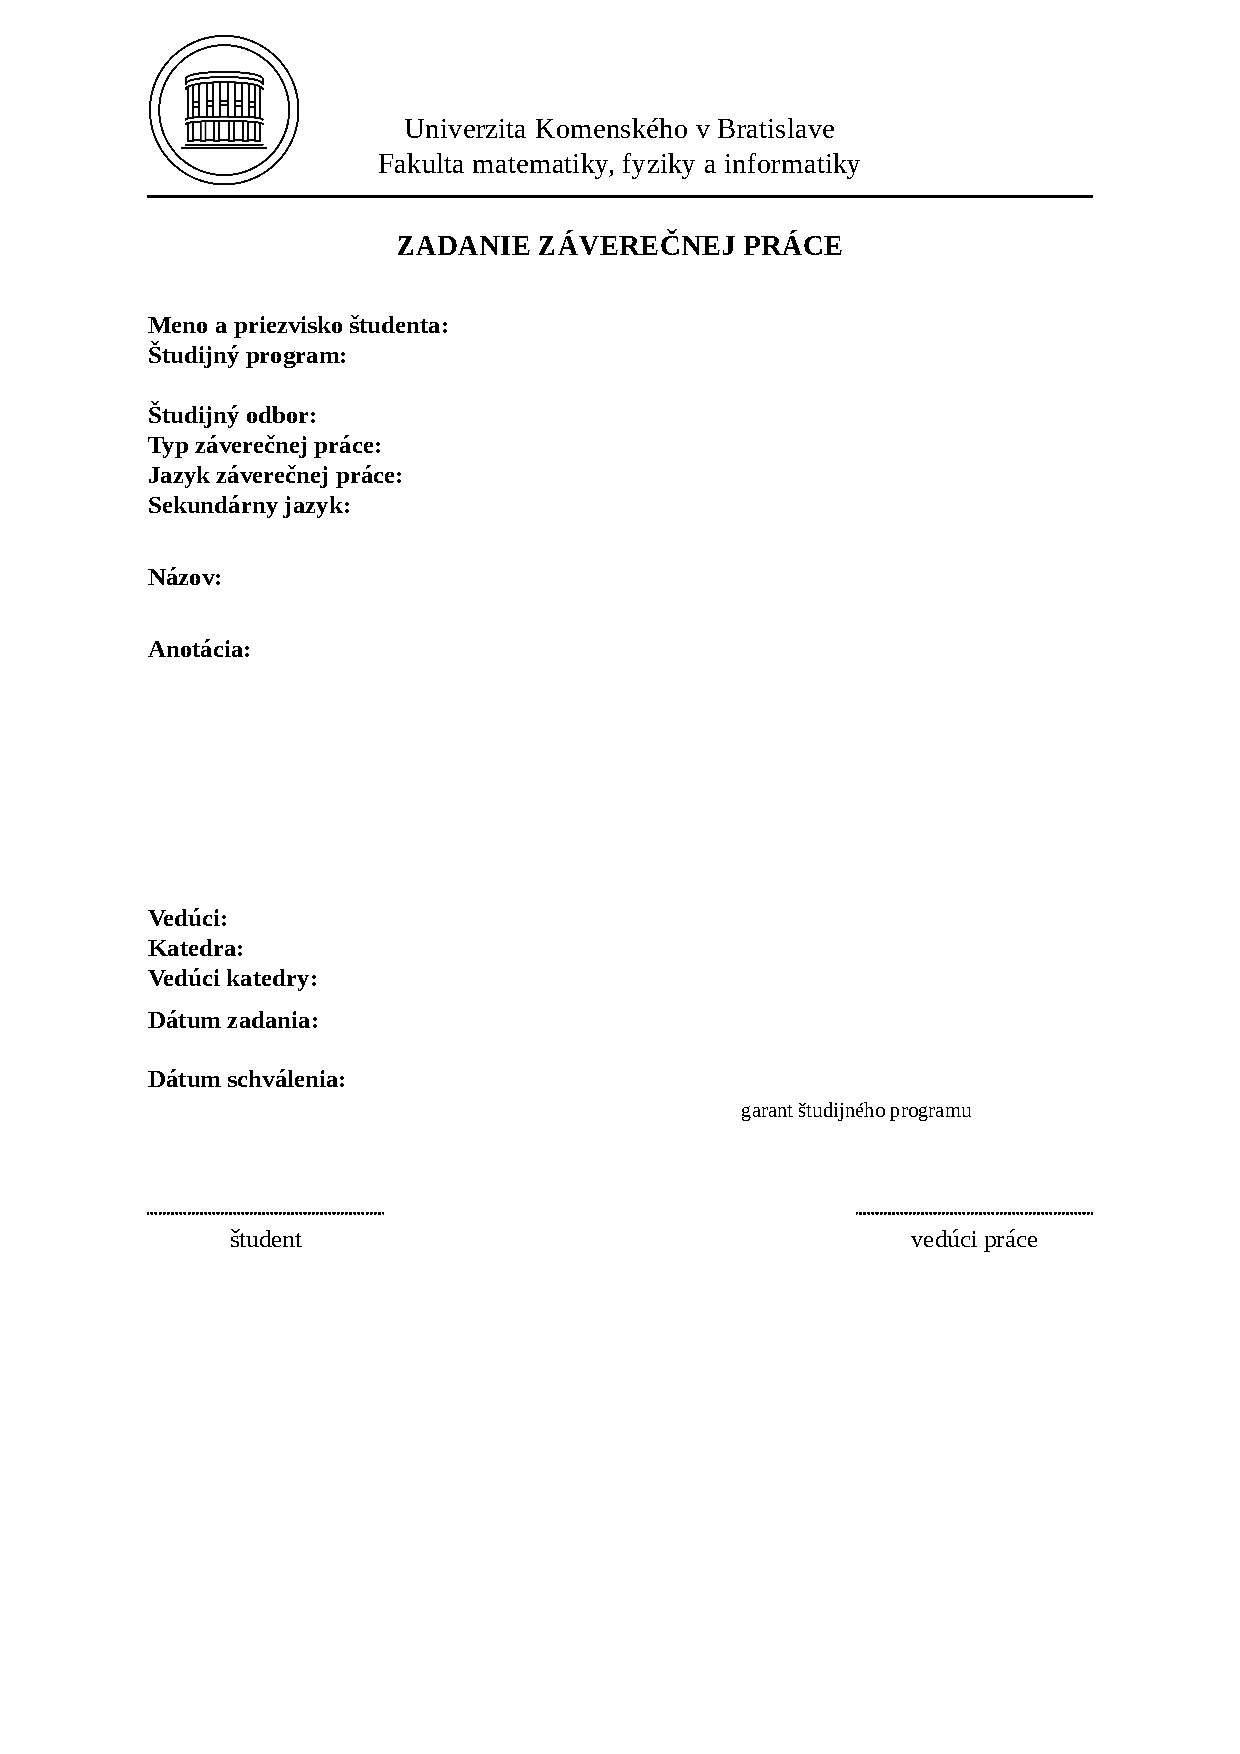
\includepdf{assignments/assignment-sk.pdf}
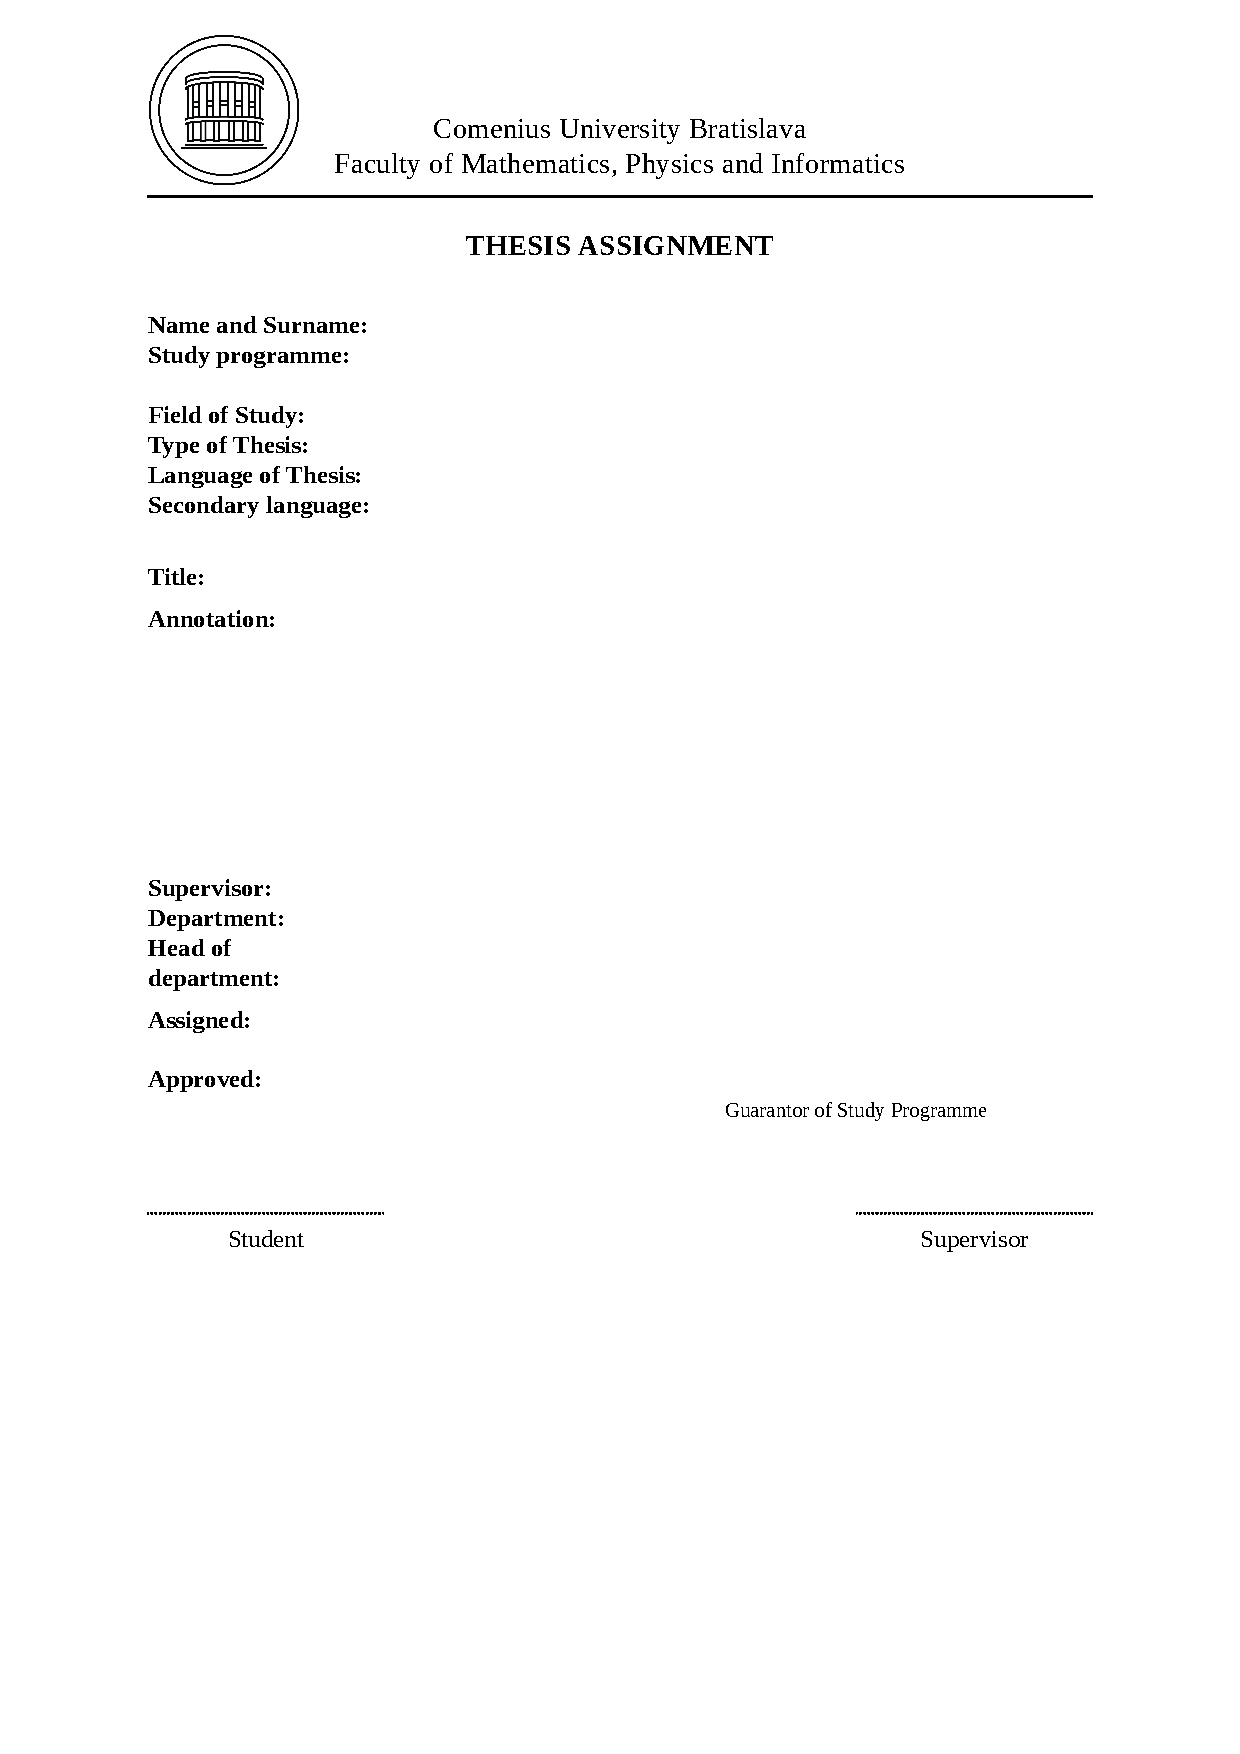
\includepdf{assignments/assignment-en.pdf}

% -------------------
% Acknowledgments (optional)
% -------------------
\newpage
\pagestyle{plain}

\vfill
{\bf Acknowledgments:} Here you can thank your supervisor and/or other persons
who somehow helped you with this thesis. You should acknowledge grants/projects
in case your research was financed by any.

% -------------------
% Abstracts (EN first, SK second)
% -------------------

\newpage 
\section*{Abstract}

English abstract: 100-500 words; keep it formatted in one paragraph.
Do not use abbreviations and other niche advanced terms here, which
will be explained in the thesis later.

\paragraph*{Keywords:} first, second, third, (fourth, fifth)

\newpage 
\section*{Abstrakt}

The Slovak abstract: should be the translation of the English one.

\paragraph*{Kľúčové slová:} jedno, druhé, tretie (prípadne štvrté, piate)

% -------------------
% Table of Contents (automatically generated)
% -------------------

\cleardoublepage 

\tableofcontents

% -------------------
% List of Figures, List of Tables (optional)
% You can also put here the List of Algorithms, Abbreviations/Acronyms, or Symbols
% if you have any
% -------------------

\newpage 

\listoffigures
\listoftables

% -------------------
% The main content body.
% You can either put everything directly here,
% but it is much cleaner to have each chapter
% in a separate file and input them here like this
% -------------------

\mainmatter
\pagestyle{headings}

\input intro.tex 

\input chapter.tex

\input conclusion.tex

% -------------------
% References (automatically generated from `references.bib`)
% -------------------


\newpage	

\backmatter

\thispagestyle{empty}
\clearpage

\bibliography{references} 

% -------------------
% Appendices (optional)
% -------------------

%\input appendixA.tex

%\input appendixB.tex

\end{document}
